\documentclass[12pt]{article}
\usepackage[authordate]{biblatex-chicago}
\addbibresource{PhDWritingSample.bib}
\usepackage{tikz}
\usepackage{booktabs}
\usetikzlibrary{trees}
\usepackage{float}
\usepackage{enumitem}
\usepackage{hyperref}
\usepackage[bottom]{footmisc}
\hypersetup{
    colorlinks=true,
    urlcolor=blue,
    linkcolor=black,
    citecolor=black
}

%------------------------------------
% PAGE LAYOUT: 1" margins, double-spaced
%------------------------------------
\usepackage[margin=1in]{geometry}
\usepackage{setspace}
\setstretch{2}
\setlength{\parindent}{0.5in}
\setlength{\parskip}{0pt}
\usepackage{titlesec}
\setcounter{secnumdepth}{0}
\titleformat{\section}
  {\normalfont\bfseries\scshape}
  {}
  {0pt}
  {}
\titlespacing*{\section}{0pt}{1ex}{0.5ex}

%------------------------------------
% META
%------------------------------------
\title{Red Lines That Bind: International Law and Domestic Political Audiences in U.S. Counterproliferation Policy}
\author{Ethan J. Lee}
\date{November 2025}

\renewcommand{\contentsname}{Table of Contents}

\begin{document}

%------------------------------------
% COVER PAGE
%------------------------------------
\begin{titlepage}
\centering
\vspace*{.25in}

{\Large Red Lines That Bind:\\[-20pt]
International Law and Domestic Political Audiences\\[-20pt]
in U.S. Counterproliferation Policy\par}

\vspace{1em}

{\textbf{Ethan J. Lee}\par}

\vspace{0.5em}

{\textbf{December 1, 2025}\par}

\vspace{2em}

\textbf{Abstract}

\vspace{0.5em}

\begin{minipage}{0.8\textwidth}
\setstretch{1.15}
\noindent
To examine when and how the stated international legality of threats shapes audience costs and their underlying mechanisms, I fielded an original vignette survey that presented a non-probability sample of U.S. adults with vignettes about a hypothetical U.S.–Iran nuclear proliferation crisis. My data indicate that legality cues can realign reputation-based mechanisms of audience costs (inconsistency and belligerence) but not the outcome-based mechanism of audience costs (incompetence). I also show that respondents high in militant assertiveness and national chauvinism are especially supportive of leaders who successfully carry out threats that are stated to be internationally unlawful, but they diverge in their levels of approval of leaders who back down from threats or stay out. The results have theoretical implications for how international legality can shape leaders’ domestic political incentives in crisis bargaining, particularly as it concerns the credibility of threats as perceived by the targets of coercion.\\
\vspace{0.5em}\\
\textbf{Author’s Note:} This is an edited version of my 2023 undergraduate thesis submitted to the Center for International Security and Cooperation’s Interschool Honors Program. The code and data used in this paper, as well as the appendix containing the survey questionnaire and a table summarizing the survey sample’s characteristics, are available at this GitHub repository: \href{https://github.com/ethanjoshlee/Red-Lines-That-Bind}{github.com/ethanjoshlee/Red-Lines-That-Bind}.
\end{minipage}

\end{titlepage}

\pagenumbering{arabic}
\setcounter{page}{1}

%------------------------------------
% MAIN TEXT
%------------------------------------

\section{Introduction}

On January 3, 2020, a U.S. drone strike killed Iranian general Qasem Soleimani in Baghdad.\footnote{\textcite{baker_seven_2020}.} Iran’s leader Ayatollah Ali Khamenei then vowed “severe revenge,” prompting U.S. President Donald Trump to respond with a threat of his own on Twitter: “if Iran strikes any Americans, or American assets, we have targeted 52 Iranian sites… some at a very high level and important to Iran and the Iranian culture, and those targets, and Iran itself, WILL BE HIT VERY FAST AND VERY HARD.”\footnote{\textcite{brown_qasem_2020, trump_iran_2020}.}

Trump’s threatened strikes drew widespread denunciation over the fact that they would have almost certainly violated both international and U.S. domestic law.\footnote{For more on whether it is internationally lawful to make a threat that would violate international law, see \textcite{sturchler_threat_2007, weiner_threating_2025}. For legal analysis of Trump’s threatened strikes, see \textcite{nevitt_trumps_2020}.} Yet after Iran launched a large ballistic missile attack against bases housing over a thousand American troops, the United States refrained from any military response, and Trump’s approval rating climbed to a personal best by the end of the month.\footnote{\textcite{chuck_ain_2020, jones_trump_2020}.} Why did Trump’s approval rating increase following the crisis?

This case points to a larger empirical puzzle: how international law shapes leaders’ political incentives in crisis bargaining. Schelling once contended that “one of the great advantages of international law and custom… is that a country may be obliged \textit{not} to engage in some dangerous rivalry when it would prefer not to but might otherwise feel obliged to for the sake of its bargaining reputation.”\footnote{\textcite{schelling_arms_1966}.} Scholars have since addressed different facets of this puzzle through largely separate literatures that examine crisis bargaining and international law compliance. Yet despite the depth of research in both of these areas of study, a key question remains unanswered: in crisis bargaining, when and how do cues about the international legality of military action affect audience cost mechanisms?

To empirically test this research question, I fielded an original vignette survey experiment in February 2023, presenting respondents with vignettes about a hypothetical U.S.–Iran nuclear proliferation crisis. The survey tested the effect of unambiguous legality cues—stating that U.S. nuclear counterproliferation strikes would either violate or not violate international law—on mechanisms underlying audience cost. My results show that legality cues can shift reputation-based audience cost mechanisms, such as inconsistency and belligerence. On the other hand, the outcome-driven dimension of audience costs (incompetence) is consistent no matter which way legality is framed, with respondents perceiving comparable levels of reputational damage. The effects of legality also vary by predispositions: respondents high in militant assertiveness and national chauvinism are especially supportive of leaders who successfully carry out threats that are stated to be internationally unlawful, yet they diverge in their approval of staying out and backing down.

My paper is organized as follows. First, I examine relevant research on audience costs, nuclear counterproliferation, and international law compliance. Drawing on this work, I propose three hypotheses about how unambiguous international legality cues can shift the underlying mechanisms of audience costs. Second, I describe the survey design and present the main findings from the experiment. Third, I analyze average treatment effects and the relationship between respondents’ individual characteristics and their levels of approval. Fourth, I conclude by summarizing my findings, discussing the implications of these results, and identifying promising avenues for future research.

\section{Literature Review and Hypotheses}

The success of interstate threats for deterrence or compellence can hinge on whether the target believes the coercing party will prefer carrying out the threatened action to backing down.\footnote{\textcite{schelling_arms_1966}.} That belief depends, in part, on perceptions of the leader’s resolve and the relative political costs of following through versus reneging.\footnote{\textcite{lebow_between_1984}.} Because only leaders themselves know their true resolve in crisis bargaining—creating incentives for parties to exaggerate—classic crisis-bargaining theory holds that leaders can make threats credible by taking costly steps that they would only be willing to incur if resolved.\footnote{\textcite{schelling_strategy_1960, fearon_rationalist_1995, fearon_signaling_1997}.} Audience cost theory extends this logic to the internal politics of states: by issuing public threats, leaders can expose themselves to potential domestic political punishment if they renege. Anticipating these internal political incentives, foreign targets may view such threats as more credible.\footnote{\textcite{fearon_domestic_1994, fearon_signaling_1997}.}

% \footnote{\textcite{}.}

Because the logic of audience cost theory is subject to selection bias—leaders may issue threats only if they are serious about following through—scholars have relied on surveys to test and observe them.\footnote{\textcite{schultz_looking_2001, snyder_cost_2011, tomz_domestic_2007}.} For canonical “repel-the-invader” experiments, participants read a vignette in which an unnamed state attacks its neighbor. The control describes a president who commits to staying out of the conflict, while the treatment describes a president who publicly makes a compellent threat to intervene but then does not follow through. By comparing respondents’ levels of political support for the president across these conditions, scholars have found that reneging on public threats can result in lower political support for the president. Scholars have taken this relative decrease as evidence of audience costs.\footnote{\textcite{tomz_domestic_2007}.}

While early studies theorized that audience costs arise as a response to inconsistency—with citizens punishing leaders for the gap between words and actions, fearing damage to their country’s reputation for resolve—more recent research has shown that inconsistency is not the only mechanism underlying audience costs.\footnote{\textcite{fearon_domestic_1994, tomz_domestic_2007, levendusky_when_2012, kertzer_decomposing_2016, evers_is_2019, lin-greenberg_backing_2019}.} By utilizing experiments with conditions in which leaders actually carry out their threats, scholars have demonstrated the existence of “belligerence costs,” whereby some respondents penalize leaders for making a threat in the first place.\footnote{\textcite{kertzer_decomposing_2016, nomikos_what_2019}.} Another audience cost mechanism distinct from reputational concerns involves perceptions of competence: whether a leader is capable of achieving desirable or expected policy outcomes.\footnote{\textcite{smith_international_1998, schultz_democratic_1999, ramsay_politics_2004, gelpi_competency_2015}.} Research has demonstrated that incompetence costs—measured by looking at how much support leaders get when they follow through and fail compared to when they succeed—were often inadvertently bundled into earlier studies' measures of inconsistency and belligerence.\footnote{\textcite{nomikos_what_2019}.} Indeed, strong dispositions regarding competence can dampen penalties for inconsistency.\footnote{\textcite{chaudoin_promises_2014}.}

In standard repel-the-invader vignettes, intervention is prima facie legitimate under the principle of collective self-defense. Yet these audience cost experiments have not tested the effect of international legality cues, leaving respondents to form their own assumptions about the lawfulness of threatened military action. To isolate the effect of legality cues on audience costs, experiments should shift away from repel-the-invader vignettes. Instead, experiments should use scenarios where legality cues are more plausibly malleable, such as nuclear counterproliferation, for which legal scholars dispute the international legality.\footnote{\textcite{arend_international_2003, spector_israels_2008, sofaer_best_2010, el_molla_prohibition_2013, sarvarian_lawfulness_2014, pulcini_ounce_2021, schmitt_israels_2025}.}

Distinct from research on audience costs is the literature examining when and why states comply with international regimes. Recent work in this field often uses survey experiments to study how international law shapes domestic public opinion.\footnote{\textcite{downs_is_1996, von_stein_treaties_2005, chilton_why_2013, morrow_order_2014, dill_legitimate_2014, fazal_wars_2018, chilton_preferences_2021, abebe_social_2021}.} In the context of armed conflict, studies have argued that cues signaling the illegality of certain policies tend to shift public preferences toward compliance with the law (though other research has contended that these effects weaken in the face of counterarguments or competing incentives).\footnote{\textcite{wallace_international_2013, kreps_international_2016, carpenter_stopping_2020, press_atomic_2013, chilton_laws_2015, sagan_revisiting_2017, sagan_just_2019, lupu_violence_2019, sagan_does_2020, dill_attitudes_2021, chaudoin_how_2023, morse_strategies_2022, dill_kettles_2022, sagan_atomic_2025}.} A separate body of doctrinal and theoretical work contends that legal threats are more credible; however, this literature is not empirical and is largely centered on nuclear threats, with key questions about the law’s effect on the credibility of threats remaining largely unanswered.\footnote{\textcite{dunlap_taming_1997, kehler_nuclear_2016, waxman_war_2018, sagan_rule_2021}.}

The audience cost literature has identified three mechanisms—inconsistency, belligerence, and incompetence—but it does not explicitly test how legality cues can influence them. By contrast, the international law compliance literature shows that legality cues can influence public support for certain foreign policies, yet it does not link these shifts to the political incentives facing leaders in crisis bargaining. This leaves a clear empirical gap: we know little about how information on legality can realign incentives in crisis bargaining, particularly audience costs and their underlying components.

\begin{figure}[H]
\centering
\setstretch{1}
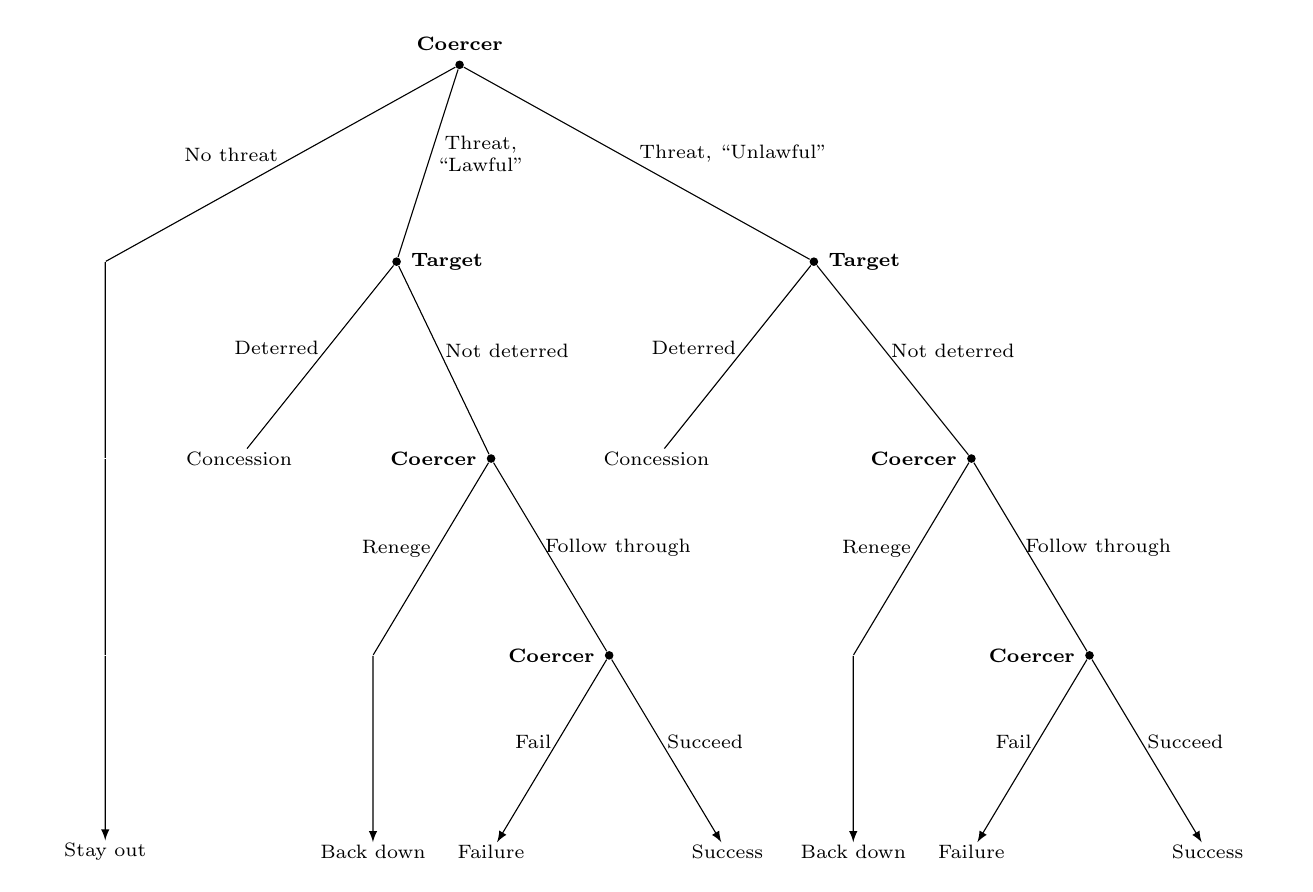
\begin{tikzpicture}[
  grow=down,
  level distance=25mm,
  sibling distance=30mm,
  every node/.style={font=\scriptsize},
  edge from parent/.style={draw},
  player/.style={circle,fill=black,inner sep=1.1pt,label distance=6pt},
  terminal/.style={align=center,inner sep=1pt,text width=1.9cm},
  dummy/.style={inner sep=0pt,minimum size=0pt,draw=none},
  level 1/.style={sibling distance=45mm},
  level 2/.style={sibling distance=40mm},
  level 3/.style={sibling distance=30mm},
  edgelabel/.style={pos=.45, above, font=\scriptsize, inner sep=0pt, align=center},
  edgelabelL/.style={edgelabel, anchor=east},
  edgelabelR/.style={edgelabel, anchor=west}
]
\node[player,label=above:\textbf{Coercer}] {}
  child { node[dummy] {}
          child { node[dummy] {}
                  child { node[dummy] {}
                          child { node[terminal] {Stay out}
                                  edge from parent[draw,-latex]
                                }
                        }
                }
          edge from parent node[edgelabelL, xshift=-7pt] {No threat}
        }
  child[xshift=-8mm] { node[player,label=right:\textbf{Target}] {}
          child { node[terminal] {Concession}
                  edge from parent node[edgelabelL, xshift=-3pt] {Deterred}
                }
          child[xshift=-8mm] { node[player,label=left:\textbf{Coercer}] {}
                  child { node[dummy] {}
                          child { node[terminal] {Back down}
                                  edge from parent[draw,-latex]
                                }
                          edge from parent node[edgelabelL, xshift=-2pt] {Renege}
                        }
                  child { node[player,label=left:\textbf{Coercer}] {}
                          child { node[terminal] {Failure}
                                  edge from parent[draw,-latex]
                                       node[edgelabelL, xshift=-2pt] {Fail}
                                }
                          child { node[terminal] {Success}
                                  edge from parent[draw,-latex]
                                       node[edgelabelR, xshift=+2pt] {Succeed}
                                }
                          edge from parent node[edgelabelR] {Follow through}
                        }
                  edge from parent node[edgelabelR, xshift=+2pt] {Not deterred}
                }
          edge from parent node[edgelabelR, xshift=+2pt] {Threat,\\``Lawful''}
        }
  child { node[player,label=right:\textbf{Target}] {}
          child { node[terminal] {Concession}
                  edge from parent node[edgelabelL, xshift=-3pt] {Deterred}
                }
          child { node[player,label=left:\textbf{Coercer}] {}
                  child { node[dummy] {}
                          child { node[terminal] {Back down}
                                  edge from parent[draw,-latex]
                                }
                          edge from parent node[edgelabelL, xshift=-2pt] {Renege}
                        }
                  child { node[player,label=left:\textbf{Coercer}] {}
                          child { node[terminal] {Failure}
                                  edge from parent[draw,-latex]
                                       node[edgelabelL, xshift=-2pt] {Fail}
                                }
                          child { node[terminal] {Success}
                                  edge from parent[draw,-latex]
                                       node[edgelabelR, xshift=+2pt] {Succeed}
                                }
                          edge from parent node[edgelabelR] {Follow through}
                        }
                  edge from parent node[edgelabelR, xshift=+2pt] {Not deterred}
                }
          edge from parent node[edgelabelR, xshift=+7pt] {Threat, ``Unlawful''}
        };
\end{tikzpicture}
\caption{Game tree of crisis outcomes for internationally ``lawful'' and ``unlawful'' cues.}
\label{fig:gametree}
\end{figure}
\setstretch{2}

Figure 1 presents a simplified crisis game, derived from the audience cost literature, that incorporates unambiguous legality cues tied to the leader’s threatened military action. The coercing party first decides whether to issue a deterrent threat, with context provided on whether the threatened action is lawful or unlawful under international law. If the target is not deterred by the threat, the leader must then choose between following through or backing down, and, if the leader follows through, the military action may either succeed or fail to achieve stated objectives. I can use the distinct outcomes at the end of these paths to measure the effect of legality cues on inconsistency, belligerence, and incompetence costs.

Unambiguous legality cues can provide individuals with a heuristic for evaluating the legitimacy and potential reputational consequences of threatened military action. If the vignette frames the action as permissible under international law, respondents will tend to see it as justified, leading many to view backing down as abandoning a legitimate commitment. This motivates Hypothesis 1a: \textit{when military action is described as lawful, there will be an inconsistency cost}. By contrast, if a vignette describes threatened military action as a violation of international law, carrying it out would constitute an illegal act. Since many would then likely view backing down as protecting the nation’s standing, there should be an increase in average support for backing down relative to following through. This leads to Hypothesis 1b: \textit{when military action is described as unlawful, there will be an inconsistency benefit}.

A similar logic extends to belligerence. When a vignette describes threatened military action as internationally lawful, individuals should be more likely to interpret carrying out the threat as a justified use of force rather than as a gratuitous escalation. On average, this should increase support for a leader who engages relative to one who stays out. This leads me to Hypothesis 2a: \textit{when military action is described as internationally lawful, there will be a belligerence benefit}. Conversely, when a vignette describes threatened military action as unlawful, making and then carrying out the threat is more likely to be viewed as unwarranted aggression that breaks international norms and hurts the country’s reputation. Under these conditions, average support should be higher for staying out than for following through. Hence, Hypothesis 2b: \textit{when military action is described as internationally unlawful, there will be a belligerence cost}.

In contrast to public perceptions of inconsistency and belligerence, which are largely rooted in concerns about reputation, incompetence costs arise from a mismatch between outcomes and the public’s preferred or expected policy goals. Even when military action purportedly complies with international law, failure can make leaders look incompetent. Conversely, a supposedly illegal operation that succeeds might be seen as having secured an important foreign policy win. This means that individuals are more likely to penalize unsuccessful operations than successful ones, regardless of whether the action is stated to be legal or illegal. This logic provides the basis for Hypothesis 3: \textit{there will be incompetence costs regardless of whether military action is described as internationally lawful or unlawful}.

\section{Experimental Design}

To test these hypotheses, I fielded a vignette survey in February 2023 that presented participants with vignettes about a hypothetical U.S.–Iran nuclear proliferation crisis.\footnote{I explicitly referenced Iran instead of an unidentified state to prevent respondents from speculating and to enhance external validity by situating the vignette in a plausible scenario. For more on country names and trade-offs with abstraction in vignette survey experiments, see \textcite{dafoe_information_2018, majnemer_names_2022, brutger_abstraction_2023}.} I used Lucid (then a Cint Group company) to recruit a non-probability sample of U.S. adults demographically representative of the American public in terms of age, gender, race and ethnicity, income level, and region. A total of 2,521 respondents completed the survey, with approximately 350 in each of the seven experimental conditions (one control and six treatments).

Across all of the experiment’s conditions, respondents first read that Iran has enough nuclear material to construct a nuclear weapon and that leaders from both major U.S. political parties have expressed concern. The control then reports that an unnamed U.S. president said the United States would not become involved. In each treatment, by contrast, respondents read that the president “publicly stated that if Iran conducted a nuclear weapons test, the U.S. military would use conventional (non-nuclear) weapons specifically to destroy all of Iran’s nuclear weapons facilities,” with the threatened attack primed as either violating or not violating international law. After presenting this initial background, the control and treatments alike state that Iran conducted a nuclear weapons test. The treatment vignettes then vary in two additional respects: whether the president followed through on the threat or backed down, and, if the president followed through, whether the U.S. military operation succeeded or failed to destroy Iran’s nuclear facilities.\footnote{See the appendix for more details on the survey design, vignettes, and characteristics of the survey sample.}

\vspace{16pt}

\begin{table}[H]
\centering
\label{tab:treatments}
\begin{tabular*}{\textwidth}{@{\extracolsep{\fill}}lccc}
\hline
 & \small{Follow Through, Success} 
 & \small{Follow Through, Failure} 
 & \small{Back Down} \\
\hline
\small{Internationally Lawful}   
  & \small{Treatment 1} 
  & \small{Treatment 2} 
  & \small{Treatment 3} \\
\small{Internationally Unlawful} 
  & \small{Treatment 4} 
  & \small{Treatment 5} 
  & \small{Treatment 6} \\
\hline
\end{tabular*}

\vspace{0.5em}

\begin{minipage}{\textwidth}
\footnotesize \emph{Note:} This table does not include the control condition, in which the president stated that the United States would not intervene.
\end{minipage}
\caption{The survey experiment’s six treatment conditions.}
\end{table}

After respondents read the full vignette and completed a reading check, they indicated their level of approval for the president’s decision on a six-point Likert scale.\footnote{The survey included a reading check that offered respondents two opportunities to correctly identify the countries mentioned in the scenario (the United States and Iran), with those who failed both attempts being removed from the study.} I use these approval levels—ranging from strongly disapprove to strongly approve—as the experiment’s primary dependent variable, estimating each audience cost mechanism by comparing mean approval across the relevant conditions. To examine heterogeneity in respondent reactions, my survey also included items to measure individual dispositions and attitudes. In particular, I asked respondents to estimate the extent of reputational damage the United States would incur in the scenario assigned to them, from “none at all” to “a great deal.”\footnote{I also asked respondents to assess the reputational consequences for the president, but, similar to \textcite{brutger_dispositional_2018}, I find no meaningful difference between these two measures. For that reason, I report results using the measure of perceived reputational damage to the United States.} I also asked a battery of questions to assess political dispositions commonly used in political psychology research. This included measures of each respondent’s militant assertiveness and national chauvinism, which capture variation in preferences for using military force over diplomacy and in sentiments of national superiority accompanied by distrust or hostility toward outgroups, respectively.\footnote{\textcite{de_figueiredo_are_2003, kertzer_decomposing_2016}.}

To test for inconsistency costs and benefits, as well as perceived reputational consequences for inconsistency, I compare mean approval for backing down (Treatments 3 and 6) with mean approval for following through on the threat and failing (Treatments 2 and 5). To test for belligerence costs and benefits, as well as perceived reputational consequences for belligerence, I similarly compare following through and failing (Treatments 2 and 5) with the control, in which the president never issued a threat. To test for incompetence costs and benefits, as well as perceived reputational consequences for incompetence, I compare successfully following through (Treatments 1 and 4) with unsuccessfully following through (Treatments 2 and 5).\footnote{This method for measuring audience cost mechanisms is adapted from \textcite{nomikos_what_2019}.}

\vspace{16pt}

\begin{table}[H]
\centering
\begin{tabular*}{\textwidth}{@{\extracolsep{\fill}}lcc}
\hline
 & \small Internationally Lawful & \small Internationally Unlawful \\
\hline
\small Audience Costs 
  & \small Treatment 3 -- Control 
  & \small Treatment 6 -- Control \\
\small Inconsistency Costs 
  & \small Treatment 3 -- Treatment 2 
  & \small Treatment 6 -- Treatment 5 \\
\small Belligerence Costs 
  & \small Treatment 2 -- Control 
  & \small Treatment 5 -- Control \\
\small Incompetence Costs 
  & \small Treatment 2 -- Treatment 1 
  & \small Treatment 5 -- Treatment 4 \\
\hline
\end{tabular*}
\caption{Measuring effects of legality priming on audience cost mechanisms.}
\label{tab:components}
\end{table}

\section{Results}

\begin{figure}[H]
\centering
\includegraphics[width=0.95\linewidth]{Figure_DiffMeans_Approval_Relative_to_Control_Percent.png}
\caption{Average treatment effects on approval relative to the control.}
\label{fig:diffmeans-approval}
\end{figure}

\begin{table}[H]
\centering
\setstretch{1}
\begin{tabular*}{\textwidth}{@{\extracolsep{\fill}}lcc}
\hline
 & Lawful cue & Unlawful cue \\
\hline
Audience Cost (Back down vs No Threat) 
  & $0.653$ & $0.049$ \\
Inconsistency (Back down vs Fail) 
  & $<0.001$ & $0.004$ \\
Belligerence (Fail vs Control) 
  & $<0.001$ & $0.359$ \\
Incompetence (Fail vs Success) 
  & $<0.001$ & $0.006$ \\
\hline
\end{tabular*}

\vspace{0.5em}

\begin{minipage}{\textwidth}
\footnotesize
\emph{Note:} Entries are $p$-values from pairwise $t$-tests.
\end{minipage}

\caption{Key pairwise comparisons of approval across experimental conditions.}
\label{tab:pairwise-simple}
\end{table}

Figure 2 plots each treatment group’s mean approval score relative to the control, providing an overview of how approval levels shift across the seven scenarios. Table 3 complements this figure by reporting key pairwise comparisons—split by legality cue—testing audience costs and underlying mechanisms. Respondents show the highest mean approval in Treatment 1, where the President followed through on a threat to take internationally lawful military action and succeeded, and in Treatment 2, where the President followed through on the same threat but failed. Approval is lowest in Treatment 5, where the President carried out a threat with an unlawful cue and failed; in Treatment 3, where the President backed down from a threat with a lawful cue; and in the control, where the President stayed out. The statistically significant difference between backing down from a threat with an unlawful cue (Treatment 6) and backing down from a threat with the lawful cue (Treatment 3) demonstrates that the unlawful cue in Treatment 6 results in a relative benefit.\footnote{$p < 0.02$.} It is also notable that following through on a threat described as unlawful and succeeding (Treatment 4) is statistically indistinguishable from backing down from the same threat (Treatment 6), suggesting that an unambiguous illegality can collapse the distinction between following through and succeeding and backing down.

In prior repel-the-invader experiments, respondents consistently impose audience costs by punishing the leader for backing down compared to staying out. With my experiment, however, approval for backing down from a threat with a lawful cue (Treatment 3) is statistically indistinguishable from the control, and backing down from a threat with an unlawful cue (Treatment 6) yields an observably higher approval than the control.\footnote{The difference in mean approval between Treatment 3 and the control is not statistically significant ($p \approx 0.65$). By contrast, the difference between Treatment 6 and the control is statistically significant ($p < 0.05$).} This absence of audience costs likely reflects two features of the survey design. First, the legality cues embedded in the back down conditions make it difficult to directly disentangle the effects of the president’s decision-making and the legality cues. Second, in canonical repel-the-invader experiments, the control describes a president who simply states that the country “would stay out of the conflict.”\footnote{\textcite{tomz_domestic_2007}.} In my survey’s control, by contrast, the president publicly states that the country “would stay out and not intervene… [if Iran] conducted a nuclear weapon test.” For counterproliferation threats, a more analogous scenario might be a president who issued only a vague commitment to pursuing non-military options, avoiding any ex ante promise for restraint.\footnote{For new experimental research that employs a survey design with an alternative control and conditions in the context of nuclear counterproliferation threats, see \textcite{leesagan_counterproliferation_2025}.}

\begin{figure}[H]
\centering
\includegraphics[width=0.95\linewidth]{Figure_Inconsistency_Approval_Percent.png}
\caption{Effects of inconsistency on approval under lawful and unlawful legality cues.}
\label{fig:inconsistency-approval}
\end{figure}

Figure 3 captures the effect of inconsistency by visualizing the difference in mean approval between backing down (Treatments 3 and 6) and following through and failing (Treatments 2 and 5). For threats with the lawful cue, the point estimate is negative: backing down from a threat with a lawful cue is less popular than following through and failing, indicating an inconsistency cost. For threats with the unlawful cue, the estimate is positive: respondents reward the president for reneging on a threat with an unlawful cue relative to carrying it out and failing, indicating an inconsistency benefit. In short, my data are consistent with Hypotheses 1a and 1b: priming on international legality can flip the direction of the inconsistency effect, with lawful cues producing a cost for backing down and unlawful cues producing a benefit.

\begin{figure}[H]
\centering
\includegraphics[width=0.95\linewidth]{Figure_Reputation_Inconsistency_Percent.png}
\caption{Effects of inconsistency on perceived reputational damage under lawful and unlawful legality cues.}
\label{fig:inconsistency-reputation}
\end{figure}

Figure 4 helps clarify approval levels for inconsistency by repeating the comparison using perceived reputational damage. Because the dependent variable in this figure measures perceived damage on an increasing scale rather than political approval on a disapproval–approval scale, positive values indicate that respondents view inconsistency as damaging to the country’s reputation, while negative values indicate the opposite. Because this data follows the same trend as the approval, with respondents perceiving inconsistency as harming the country’s reputation when the threat is framed as legal and vice versa, the data suggest that unambiguous legality cues can help respondents make quick judgments about whether reneging hurts or protects national reputation.

\begin{figure}[H]
\centering
\includegraphics[width=0.95\linewidth]{Figure_Belligerence_Approval_Percent.png}
\caption{Effects of belligerence on approval under lawful and unlawful legality cues.}
\label{fig:belligerence-approval}
\end{figure}

\begin{figure}[H]
\centering
\includegraphics[width=0.95\linewidth]{Figure_Belligerence_Reputation_Percent.png}
\caption{Effects of belligerence on perceived reputational damage under lawful and unlawful legality cues.}
\label{fig:belligerence-reputation}
\end{figure}

Figure 5 plots the effect of belligerence as the difference in mean approval between following through and failing (Treatments 2 and 5) and staying out (the control), while Figure 6 repeats the same comparison using perceived reputational damage. For threats with a lawful cue, the approval point estimate is positive—a belligerence benefit consistent with Hypothesis 2a—and the corresponding reputational estimate is statistically indistinguishable from zero. This absence of reputational cost is consistent with the pattern of higher approval for lawful engagement.

For threats with an unlawful cue, by contrast, the belligerence point estimate for approval is not statistically significant, providing no support for Hypothesis 2b.\footnote{The belligerence estimate for approval under the unlawful cue is not statistically significant ($p \approx 0.36$).} Yet the reputational estimate is clearly positive, indicating a reputational cost to belligerence when the threatened action is framed as internationally unlawful. Even though following through on a threat with an unlawful cue does not produce a detectable belligerence cost in approval, respondents nonetheless perceive it as harming the United States’ reputation.

\begin{figure}[H]
\centering
\includegraphics[width=0.95\linewidth]{Figure_Incompetence_Approval_Percent.png}
\caption{Effects of incompetence on approval.}
\label{fig:incompetence-approval}
\end{figure}

\begin{figure}[H]
\centering
\includegraphics[width=0.95\linewidth]{Figure_Incompetence_Reputation_Percent.png}
\caption{Effects of incompetence on perceived reputational damage.}
\label{fig:incompetence-reputation}
\end{figure}

Figure 7 shows the effect of incompetence as the difference in mean approval between following through and failing (Treatments 2 and 5) and following through and succeeding (Treatments 1 and 4), while Figure 8 repeats this comparison using perceived reputational damage. Across both legality cues, failure lowers approval relative to success by a similar amount, and the overlapping confidence intervals suggest no meaningful difference in incompetence costs by international legality. In addition, neither legality cue shows a statistically significant increase in perceived reputational damage at the 0.10 level. These patterns are consistent with Hypothesis 3: respondents consistently punish leaders for incompetence regardless of differing legality cues, with legality playing no observable role in shaping reputational judgments. This is in contrast with the results for inconsistency and belligerence, for which unambiguous legality cues more systematically realigned both approval and perceived reputational damage.

\begin{figure}[H]
\centering
\includegraphics[width=1\linewidth]{Figure_MilAssert_Chauvinism_Approval.png}
\caption{Predicted approval by condition and levels of militant assertiveness and national chauvinism.}
\label{fig:milassert-chauvinism}
\end{figure}

To assess how individual predispositions contribute to these results, Figure 9 shows, for each experimental condition, the estimated association between militant assertiveness or national chauvinism and approval in each condition. Higher scores on both traits are correlated with greater overall approval for the president,\footnote{Both militant assertiveness and national chauvinism are positively associated with approval across the full sample ($p < 0.05$ for each).} particularly when the president follows through and succeeds on a threat with an unlawful cue (Treatment 4).

The two dispositions diverge, however, in conditions where the president either did not make a threat or did not follow through. When the president stays out (control) or backs down (Treatments 3 and 6), higher militant assertiveness is associated with lower approval, whereas higher national chauvinism is associated with increased approval for staying out and for backing down from a threat with an unlawful cue (Treatment 6). This suggests that underlying predispositions shape how respondents interpret both legality cues and crisis outcomes. Those who score high on militant assertiveness care most about resolve and willingness to use force, regardless of legality. Individuals with high national chauvinism, on the other hand, are especially likely to support successful unlawful strikes, but they are also more willing to approve of backing down if they perceive it as a way to save face through legal justification.

\section{Conclusion}

This paper tests when and how cues about the international legality of military action shape the mechanisms that produce audience costs. Using an original vignette survey of a hypothetical U.S.–Iran nuclear proliferation crisis with unambiguous legality cues, I show that legality cues can realign underlying audience cost components. More specifically, legality cues can reshape inconsistency costs, producing a benefit for backing down when the threat is described as internationally unlawful. Legality cues can also shift belligerence, creating a benefit for following through when military action is described as lawful under international law. In contrast, legality cues do not have disparate effects on incompetence: respondents impose costs for failure relative to success, regardless of the stated international legality of military action.

The survey data suggest these patterns arise because unambiguous legality cues give citizens a shortcut for judging what is reputationally costly or beneficial. When threatened action is framed as internationally lawful, individuals are more likely to view following through as enforcing a legitimate commitment, while backing down looks like failing to uphold a legitimate commitment. When threatened action is framed as internationally unlawful, the same behaviors reverse in meaning, and individuals tend to view not following through as avoiding a wrongful act and protecting the nation’s international standing. As a result, different legality cues reshape reputation-based mechanisms underlying audience costs—inconsistency and belligerence—but not incompetence, which is more outcome-based. The data also show that these effects are filtered through individual-level predispositions. In this experiment, I measure militant assertiveness and national chauvinism. Respondents who indicate high levels of either trait are more supportive of successful unlawful strikes, but they diverge when the president stays out or backs down: highly militant respondents tend to punish backing down, whereas highly chauvinist respondents are more willing to confer a benefit for backing down.

The central finding of this paper, that international legality cues can shift audience cost mechanisms in counterproliferation crises, offers new theoretical insight as it relates to the credibility of threats and the politics of international law compliance. If a president issues a public threat to carry out military action that unambiguously violates international law, it is possible that the threat would not generate an audience cost. This would mean that a president can back away without the public imposing a political penalty. Under the basic assumptions of audience cost theory, however, removing that penalty would weaken the perceived credibility of the threat and undermine its efficacy for deterrence or compellence.

My results point to several promising avenues for future experimental research, three of which I raise here. First, audience cost experiments should use alternative vignettes to test audience cost mechanisms in contexts beyond repel-the-invader or nuclear counterproliferation scenarios. After all, nuclear counterproliferation is likely unique compared to other types of foreign policy crises, such as humanitarian intervention, with scholars disagreeing on the consequences of nuclear proliferation for international stability.\footnote{\textcite{gaddis_long_1986, mearsheimer_back_1990, feaver_command_1992, miller_case_1993, mearsheimer_case_1993, sagan_perils_1994, sagan_spread_2012, whitlark_nuclear_2017}.} Second, cross-national surveys should examine when and why international legality cues have different effects on audience cost mechanisms across countries. Indeed, publics outside the United States have different relationships with international law, and prior research indicates that cues signaling a government’s actions as internationally unlawful can either increase or decrease support for those policies depending on the national context.\footnote{\textcite{lupu_violence_2019}.} Third, studies should investigate how legal contestation over the domestic and international legality of threatened military action affects inconsistency, belligerence, and incompetence costs, and whether contestation by elites or external actors can amplify or dampen these mechanisms.

\pagebreak

%------------------------------------
% REFERENCES
%------------------------------------

\printbibliography

\end{document}